%!TEX root = ../thesis.tex
% Spellchecker ignore
% cSpell:ignore includegraphics, ifpdf, graphicspath, Rauschenbeutel, nanowaveguides, microresonator, signicant, nanofiber, textasciitilde, autoref
%*******************************************************************************
%****************************** Introduction ***********************************
%*******************************************************************************

\chapter*{Introduction}

% **************************** Define Graphics Path **************************
\ifpdf{}
    \graphicspath{{Introduction/Figs/Raster/}{Introduction/Figs/PDF/}{Introduction/Figs/}}
\else
    \graphicspath{{Introduction/Figs/Vector/}{Introduction/Figs/}}
\fi

One of Prof.\ Rauschenbeutel projects uses a novel type of whispering-gallery-mode (WGM)
resonator interfaced via nanowaveguides and coupled to single Rubidium atoms to carry out
experiments in the realm of Cavity Quantum Electrodynamics. The WGM resonator
is a so-called bottle-microresonator (BMR) manufactured from a standard optical glass
fiber in a heat and pull process. The light is radially confined inside the resonator by
total internal reflection and propagates along the circumference of the resonator. In such
a structure, a signicant fraction of the light field propagates in the evanescent field. By
overlapping this field with the evanescent field of an optical nanofiber, light can be coupled
into and out of the resonator very efficiently. Due to the extremely low absorption
of silica (and low surface roughness) we can produce bottle-resonators with ultra-high
optical Q-factor exceeding 10\(^{8}\). Rubidium atoms are delivered to the resonator using
an atomic fountain. When the atoms enter the vicinity of the WGM, and they are in the evanescent
field they can be coupled to the light. For the moment the atoms are only flying by the 
resonator, but only for \textasciitilde{}\SI{2}{\micro\second} and moreover the distance 
between the resonator and the atom is not controlled. This prevents the realization from 
more complicated experiments. For that reason one needs to trap the atom.
The choice made to trap the atom is to use a dipole trap (see \autoref{chap:dipole}), which
is a conservative trap. Because the atoms have a velocity dispersion, we do not know in
advance when and where the atoms enter the evanescent field. For that we need to consider that
they arrive with some kinetic energy \(\Rightarrow \text{trap depth} \gg E_{kin} \).\\
The aim of this Bachelor thesis is to elaborate all the parameters needed to realise the trap.
\vspace{\fill}
\begin{figure}[hb]
    \centering
    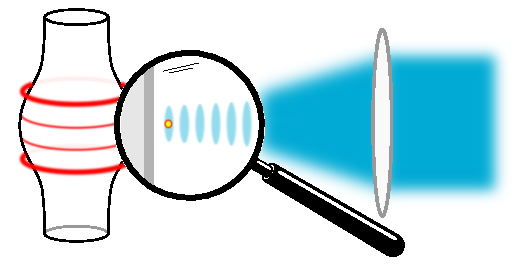
\includegraphics[width=0.6\textwidth]{resonator_trap}
\end{figure}